\documentclass[aspectratio=169, 12pt]{beamer}

% -----------------------------------------------------------------------
% Theme
% -----------------------------------------------------------------------
\usetheme{Madrid}
\usecolortheme{beaver}
\setbeamertemplate{navigation symbols}{}
\setbeamertemplate{footline}[frame number]
\setbeamerfont{frametitle}{size=\large}

% -----------------------------------------------------------------------
% Packages
% -----------------------------------------------------------------------
\usepackage{booktabs}
\usepackage{graphicx}
\usepackage{tabularx}
\usepackage{array}
\usepackage{xcolor}
\usepackage{siunitx}
\usepackage{caption}
\usepackage{subcaption}
\usepackage{amsmath}
\usepackage{hyperref}

% -----------------------------------------------------------------------
% Colors
% -----------------------------------------------------------------------
\definecolor{fireRed}{RGB}{214,39,40}
\definecolor{steelBlue}{RGB}{31,119,180}
\definecolor{forestGreen}{RGB}{44,160,44}
\definecolor{darkGray}{RGB}{80,80,80}

% -----------------------------------------------------------------------
% Paths (relative to this file in Writeup/)
% -----------------------------------------------------------------------
\graphicspath{
  {../GoogleEarth/}
  {../Analysis/data/reference/}
  {../Analysis/graphs/descriptive/}
  {../Analysis/graphs/synthetic_control/}
  {../Analysis/graphs/migration/}
  {../Analysis/graphs/commute/}
  {../Analysis/graphs/spillover/}
  {../Analysis/graphs/homelessness/}
}

% -----------------------------------------------------------------------
% Title
% -----------------------------------------------------------------------
\title[Camp Fire Economic Impacts]{
  \textbf{Economic Impacts of the 2018 Camp Fire}\\
  \normalsize Evidence from LODES Employment Data
}
\author{[Author(s)]}
\institute{[Institution]}
\date{\today}

% -----------------------------------------------------------------------
% Document
% -----------------------------------------------------------------------
\begin{document}

% --- Title slide --------------------------------------------------------
\begin{frame}
  \titlepage
\end{frame}

% --- Outline ------------------------------------------------------------
\begin{frame}{Outline}
  \tableofcontents
\end{frame}

% =======================================================================
\section{Background}
% =======================================================================

\begin{frame}{The 2018 Camp Fire}
  \begin{columns}[T]
    \begin{column}{0.55\textwidth}
      \begin{itemize}
        \item The Camp Fire ignited \textbf{November 8, 2018} in Butte County, CA
        \item Destroyed \textbf{85\%} of structures in the town of Paradise
              (pop.\ $\approx$27,000)
        \item Deadliest and most destructive wildfire in California history:
              \textbf{85 fatalities}, 18,804 structures destroyed
        \item Caused rapid displacement of nearly the entire population of Paradise
              and neighboring communities
        \item Offers a rare quasi-experimental shock to study the
              economic consequences of extreme wildfire events
      \end{itemize}
    \end{column}
    \begin{column}{0.43\textwidth}
      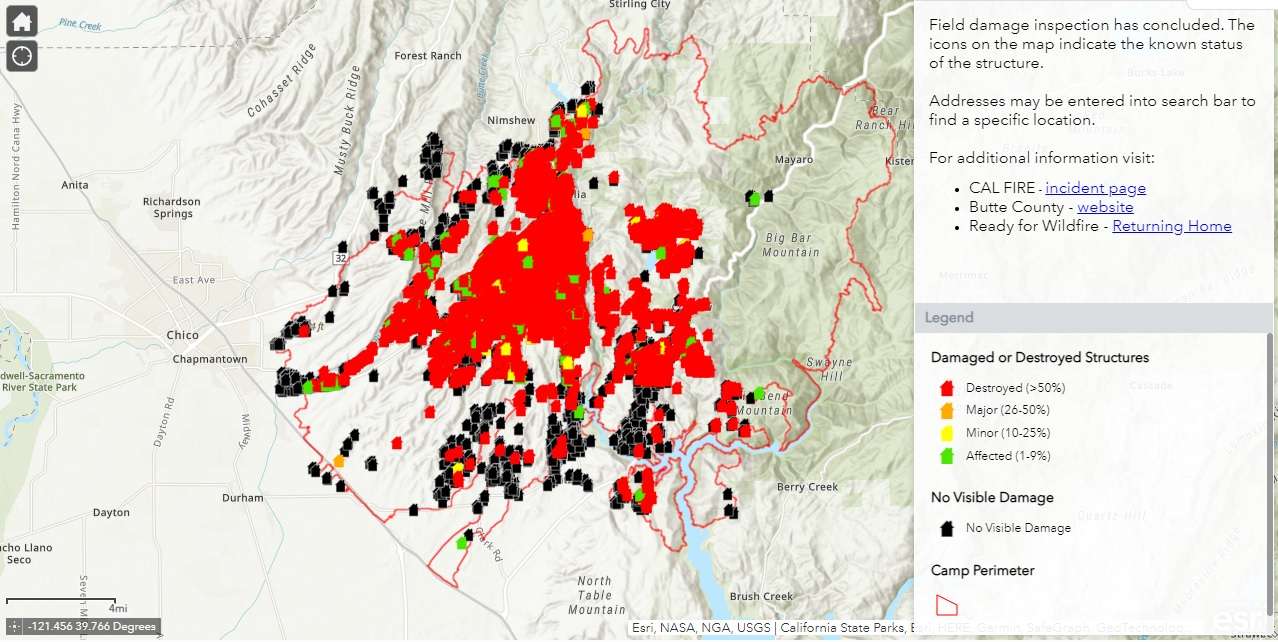
\includegraphics[width=\linewidth]{Fire_Damage_Map.jpg}
      \captionof{figure}{\footnotesize Camp Fire damage extent, Butte County}
    \end{column}
  \end{columns}
\end{frame}

% --- Google Earth imagery -----------------------------------------------
\begin{frame}{Paradise: Before and After the Fire}
  \begin{figure}
    \begin{subfigure}{0.32\textwidth}
      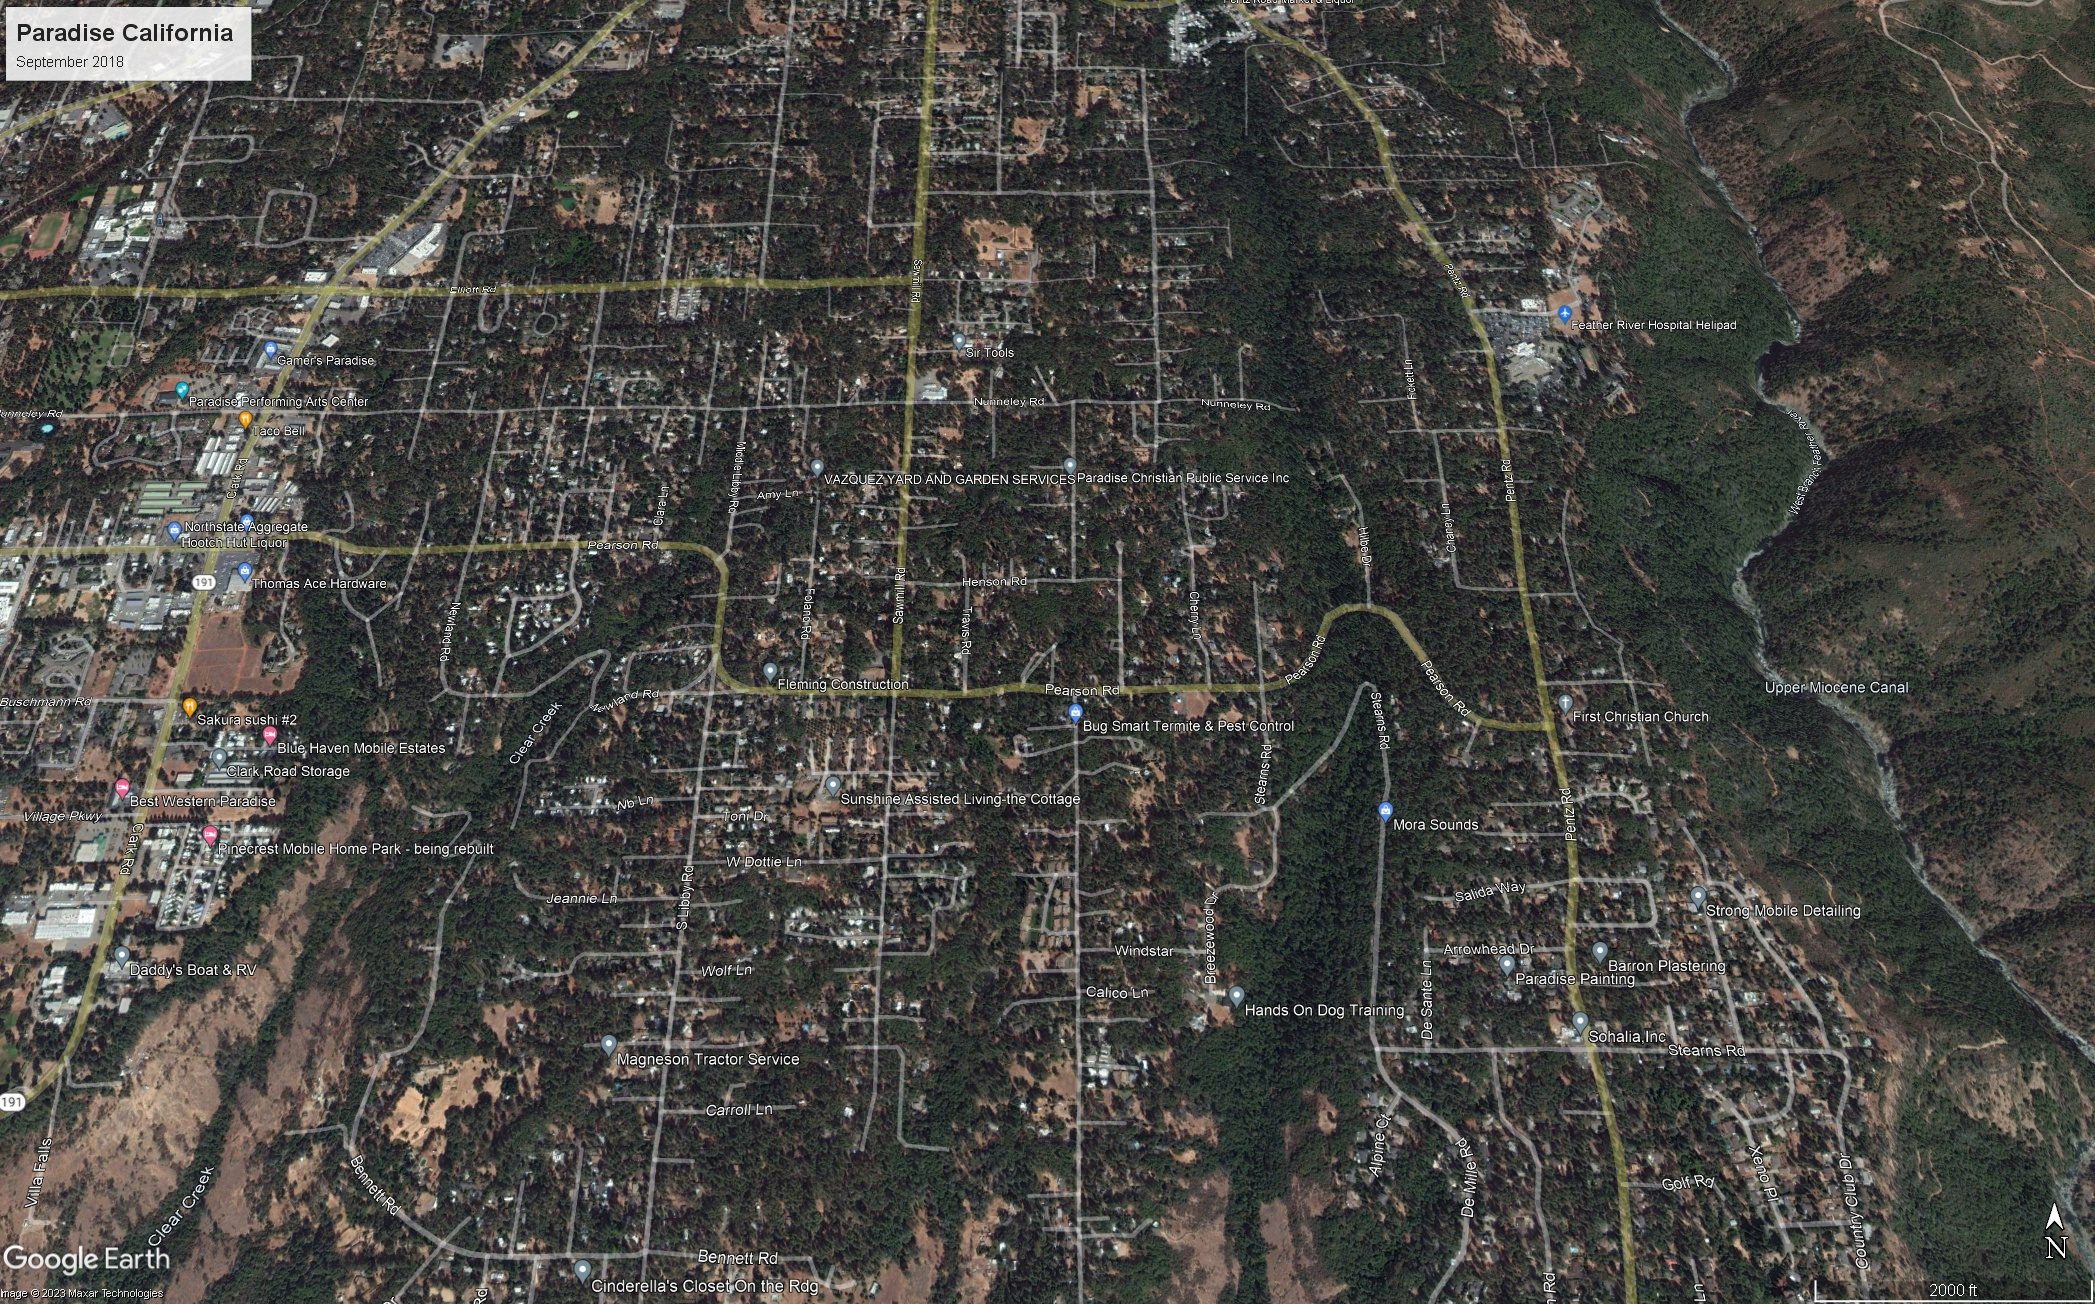
\includegraphics[width=\linewidth,height=5cm,keepaspectratio]{Paradise_Sept2018.jpg}
      \caption{\footnotesize Sept.\ 2018\\(2 months before)}
    \end{subfigure}\hfill
    \begin{subfigure}{0.32\textwidth}
      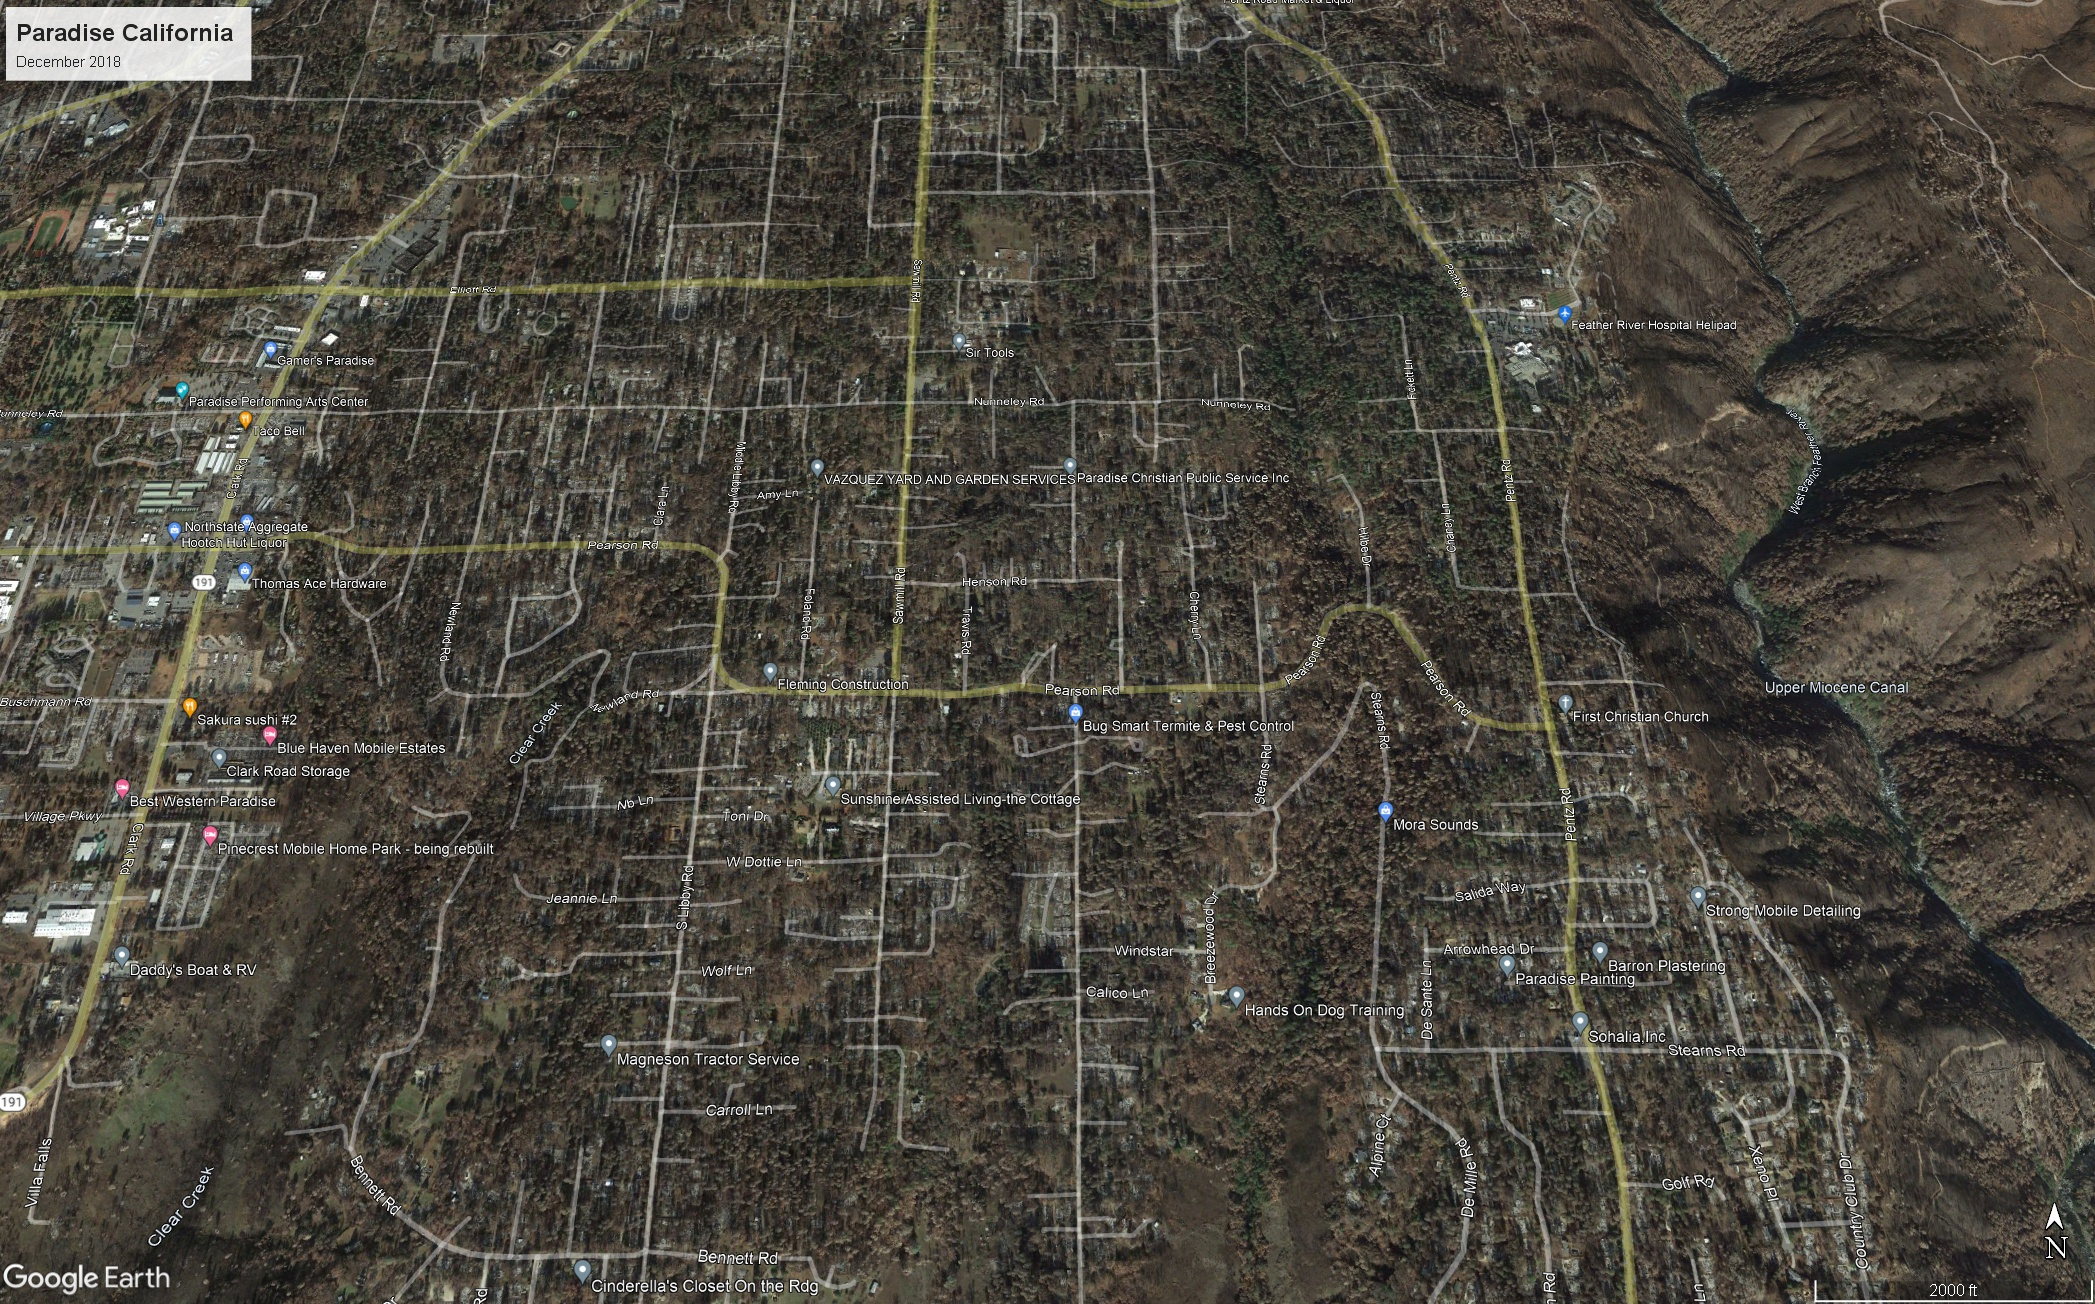
\includegraphics[width=\linewidth,height=5cm,keepaspectratio]{Paradise_Dec2018.jpg}
      \caption{\footnotesize Dec.\ 2018\\(1 month after)}
    \end{subfigure}\hfill
    \begin{subfigure}{0.32\textwidth}
      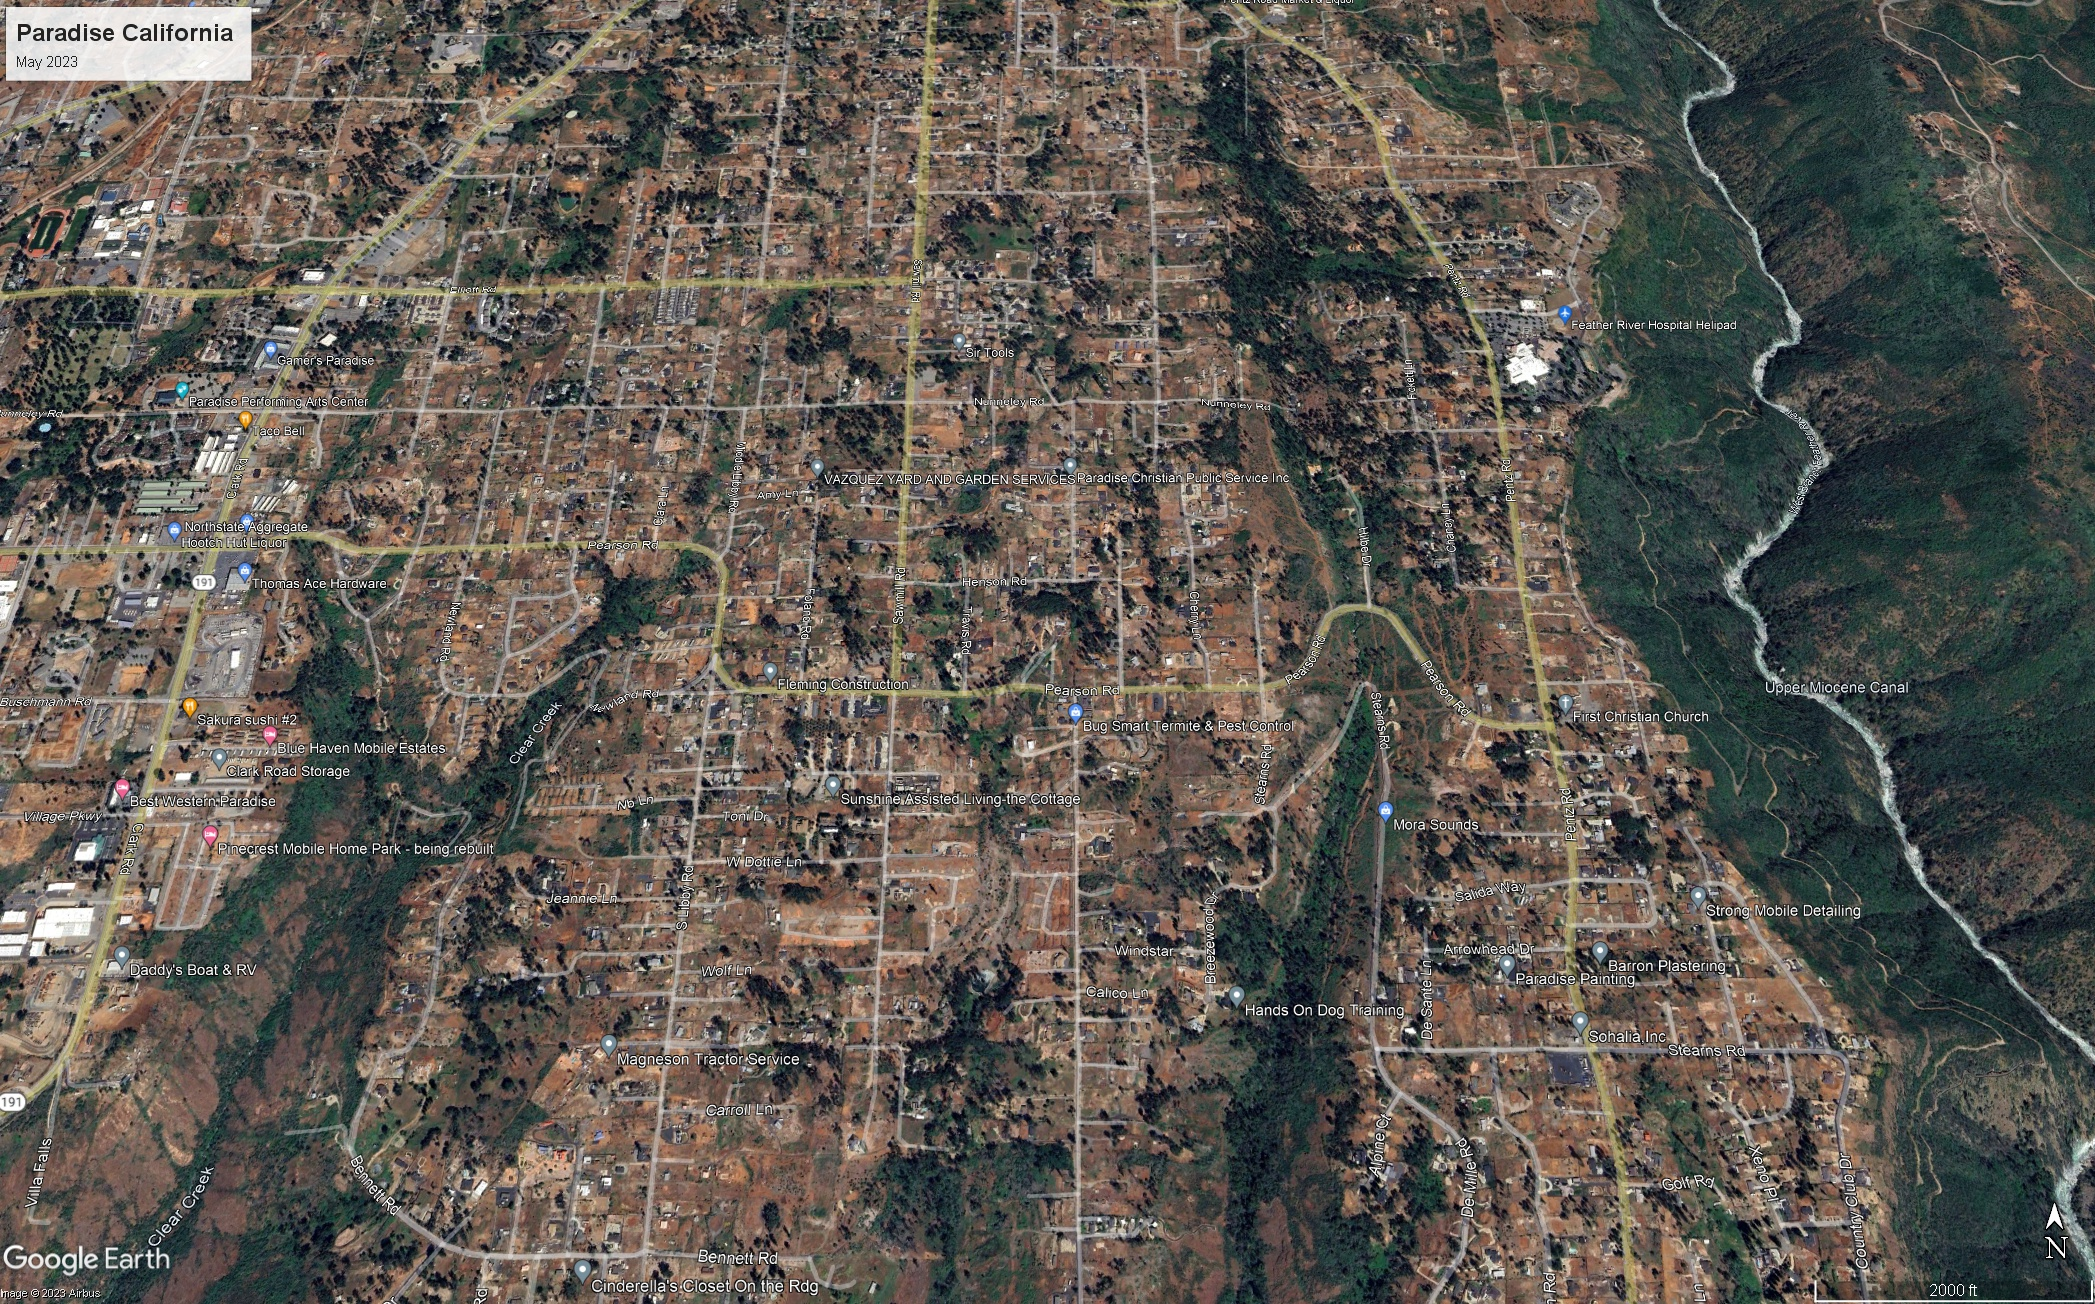
\includegraphics[width=\linewidth,height=5cm,keepaspectratio]{Paradise_May2023.jpg}
      \caption{\footnotesize May 2023\\(4.5 years after)}
    \end{subfigure}
    \caption{Google Earth imagery of Paradise, CA}
  \end{figure}
\end{frame}

\begin{frame}{Slow Recovery: Still Far Below Pre-Fire Levels}
  \begin{itemize}
    \item By 2023, \textbf{Paradise employment stood at 39\%} of its 2017 level
          (synthetic control estimate: 61\% below counterfactual)
    \item Population estimates suggest fewer than \textbf{8,000 residents}
          had returned to Paradise by 2023 (pre-fire: $\approx$27,000)
    \item Despite some rebuilding activity (construction employment up),
          the commercial and healthcare base has not returned
    \item This paper quantifies the \textbf{magnitude, sectoral composition,
          and spillover effects} of the economic shock
  \end{itemize}
\end{frame}

% =======================================================================
\section{Data and Geography}
% =======================================================================

\begin{frame}{Data Sources}
  \begin{tabular}{lll}
    \toprule
    \textbf{Dataset} & \textbf{Source} & \textbf{Coverage} \\
    \midrule
    LODES WAC/RAC & U.S.\ Census Bureau & 2013--2023, CA census blocks \\
    LODES OD & U.S.\ Census Bureau & 2013--2023, CA block-pairs \\
    IRS SOI Migration & IRS Statistics of Income & 2012--2022, county pairs \\
    USPS Vacancy & USPS / HUD & Quarterly, tract level \\
    HUD PIT Counts & HUD AHAR & 2007--2024, CoC level \\
    \bottomrule
  \end{tabular}
  \vspace{1em}
  \begin{itemize}
    \item \textbf{WAC}: Jobs by \emph{workplace} location
          (captures where people work in Paradise)
    \item \textbf{RAC}: Jobs by \emph{residence} location
          (captures where Paradise residents work)
    \item \textbf{OD}: Linked worker--workplace pairs
  \end{itemize}
\end{frame}

\begin{frame}[shrink=5]{Geographic Zones}
  \begin{columns}[T]
    \begin{column}{0.55\textwidth}
      \begin{itemize}
        \item \textbf{\color{fireRed}Paradise} (treatment): 4 census tracts\\
              {\small 06007001800, 06007001900, 06007002000, 06007002100}
        \item \textbf{Chico} (potential spillover): 25 tracts in Butte County's
              largest city, 15 miles west of Paradise
        \item \textbf{Other Butte County}: Remaining Butte County tracts
        \item \textbf{Rest of CA}: All non-Butte California tracts
              (donor pool for synthetic control)
      \end{itemize}
    \end{column}
    \begin{column}{0.43\textwidth}
      \includegraphics[width=\linewidth, height=5.5cm, keepaspectratio]{ButteCo_TractMap.pdf}
      \captionof{figure}{\footnotesize Butte County census tracts}
    \end{column}
  \end{columns}
  \vspace{0.3em}
  \footnotesize Note: Synthetic control excludes all Butte County tracts from the donor
  pool to avoid spillover contamination.
\end{frame}

% =======================================================================
\section{Methodology}
% =======================================================================

\begin{frame}{Difference-in-Differences}
  \textbf{Estimating equation} (census block $\times$ year panel, WAC and RAC):
  \[
    Y_{it} = \alpha + \beta \underbrace{(\textit{Paradise}_i \times \textit{Post}_t)}_{\text{DiD}}
           + \gamma \textit{Paradise}_i + \delta_t + \mathbf{X}_i' \boldsymbol{\phi} + \varepsilon_{it}
  \]
  \vspace{-0.5em}
  \begin{itemize}
    \item $\textit{Post}_t = 1$ for $t \geq 2019$ (fire occurred Nov 2018;
          2018 LODES is annual and partially treated)
    \item $\delta_t$: year fixed effects
    \item $\mathbf{X}_i$: 2017 baseline controls ---
          prime-age worker share, education composition, female share
    \item Standard errors \textbf{clustered at the census tract level}
    \item $\hat{\beta}$: average annual job loss per block in Paradise
          relative to the rest of Butte County
  \end{itemize}
\end{frame}

\begin{frame}{Synthetic Control}
  \begin{itemize}
    \item Creates a ``synthetic Paradise'' --- a weighted combination of
          non-Butte California tracts that best match Paradise's
          \textbf{pre-fire employment trajectory} (2013--2017)
    \item Weights chosen to minimize pre-treatment MSE;
          all data normalized to \textbf{2017 = 100}
    \item Donor pool: $\geq$500 jobs in 2017; top-500 selected by
          pre-treatment trajectory RMSE
    \item \textbf{Statistical inference}: permutation-based placebo tests ---
          apply same estimator to 100 random donor tracts and compare
          the distribution of post-treatment gaps
  \end{itemize}
\end{frame}

% =======================================================================
\section{Main Results: DiD}
% =======================================================================

\begin{frame}[shrink=20]{DiD Results: Workplace Employment (WAC)}
  \begin{table}
    \centering
    \footnotesize
    \begin{tabular}{lrrr}
      \toprule
      \textbf{Outcome} & \textbf{DiD Coef.} & \textbf{Std.\ Err.} & \textbf{p-value} \\
      \midrule
      Total Jobs          & $-26.5$\phantom{0} & $8.9$\phantom{0} & $0.003$\,*** \\
      \midrule
      \textit{By sector:} & & & \\
      \quad Retail Trade  & $-3.1$\phantom{0}  & $0.9$\phantom{0} & $<0.001$\,*** \\
      \quad Health Care   & $-18.4$\phantom{0} & $8.5$\phantom{0} & $0.030$\,**  \\
      \quad Accommodation \& Food & $-2.1$\phantom{0} & $1.0$\phantom{0} & $0.040$\,** \\
      \quad Construction  & $+0.04$            & $0.4$\phantom{0} & $0.902$       \\
      \quad Education     & $-0.1$\phantom{0}  & $1.0$\phantom{0} & $0.900$       \\
      \quad Public Admin  & $-0.1$\phantom{0}  & $0.1$\phantom{0} & $0.539$       \\
      \midrule
      \textit{By earnings:} & & & \\
      \quad Low ($\leq$\$1,250/mo)    & $-7.3$\phantom{0} & $1.8$\phantom{0} & $<0.001$\,*** \\
      \quad Medium (\$1,251--\$3,333) & $-8.4$\phantom{0} & $2.9$\phantom{0} & $0.004$\,***  \\
      \quad High ($>$\$3,333/mo)      & $-10.8$\phantom{0} & $5.3$\phantom{0} & $0.042$\,**  \\
      \bottomrule
    \end{tabular}
    \caption{DiD estimates, WAC (workplace). Controls: prime-age share,
    education composition, female share (2017 baseline). SE clustered by tract.
    $N = 20{,}885$.}
  \end{table}
\end{frame}

\begin{frame}{DiD Results: WAC vs.\ RAC}
  \begin{columns}[T]
    \begin{column}{0.5\textwidth}
      \textbf{WAC} (jobs at Paradise workplaces)
      \begin{itemize}
        \item Total: $-26.5$*** (SD $8.9$)
        \item Health Care dominates: $-18.4$**
        \item Construction: \emph{insignificant}
              (consistent with rebuilding activity)
        \item High earnings most affected in absolute terms ($-10.8$**)
      \end{itemize}
    \end{column}
    \begin{column}{0.5\textwidth}
      \textbf{RAC} (jobs held by Paradise residents)
      \begin{itemize}
        \item Total: $-24.7$*** (SD $2.3$)
        \item \emph{All} sectors and earnings tiers significant
        \item Narrower standard errors: residents dispersed to many blocks
        \item Suggests displacement was near-complete ---
              Paradise residents lost jobs across all categories
      \end{itemize}
    \end{column}
  \end{columns}
  \vspace{1em}
  \begin{block}{Key takeaway}
    Both local jobs \emph{and} employed residents were wiped out.
    The labor market disruption was total, not sector-specific.
  \end{block}
\end{frame}

\begin{frame}{Visualizing the Employment Collapse}
  \begin{figure}
    \centering
    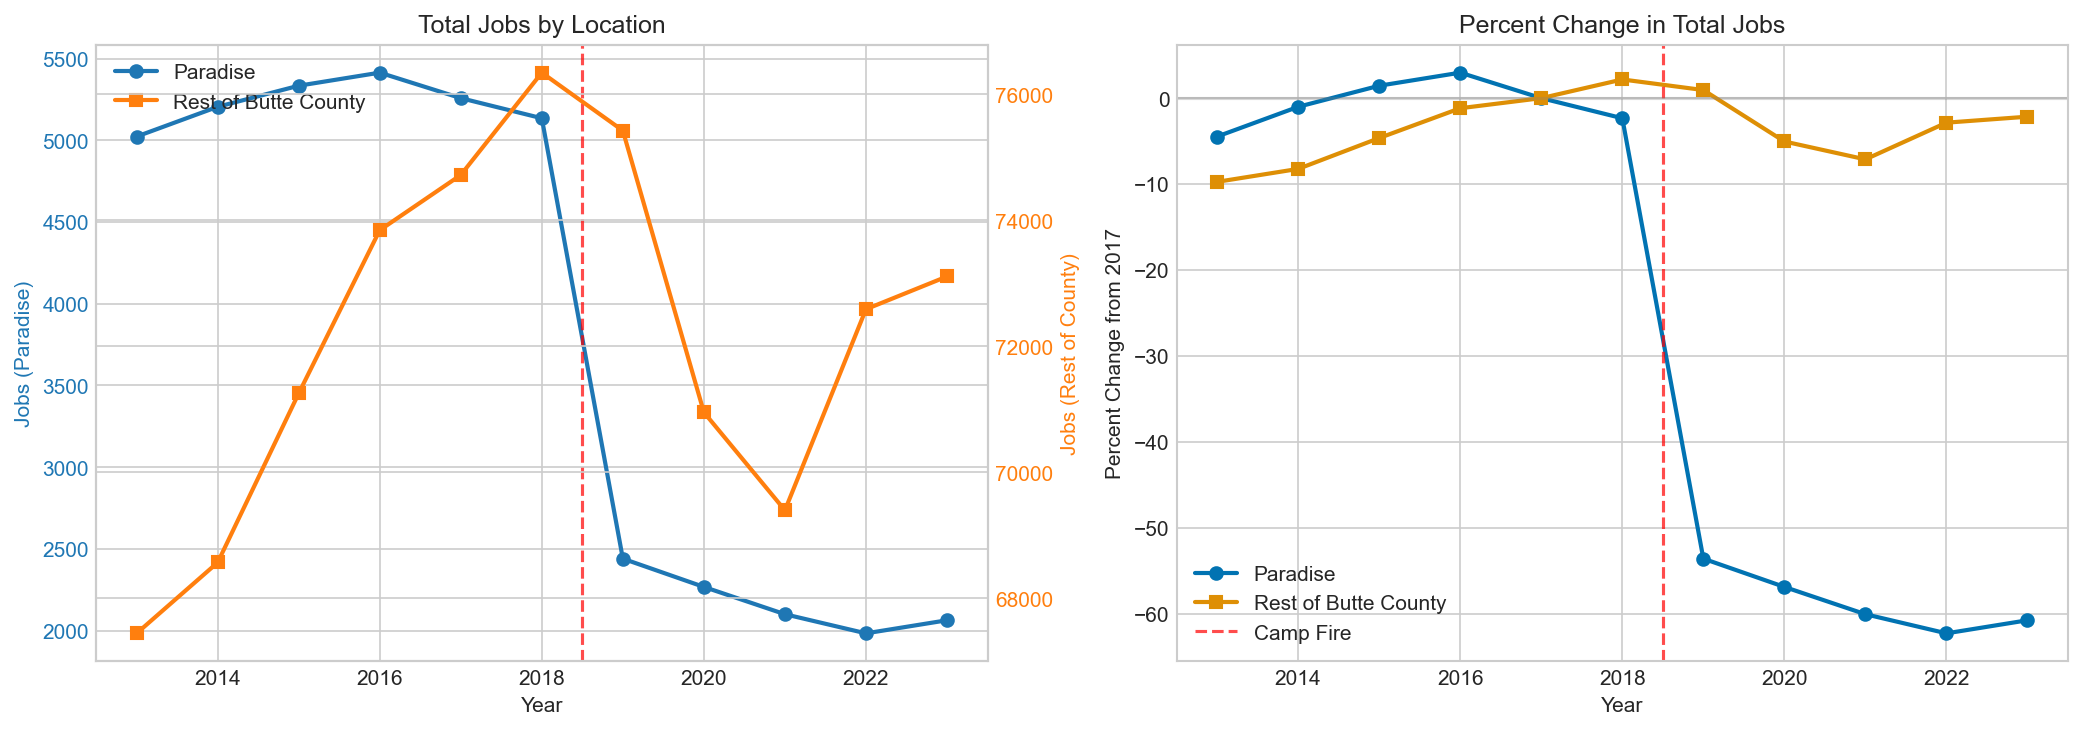
\includegraphics[width=0.85\textwidth,height=5.5cm,keepaspectratio]{total_jobs_trend_wac.png}
    \caption{Total workplace employment in Paradise vs.\ Butte County (non-Paradise),
    indexed to pre-fire trends. Vertical line: Camp Fire (Nov 2018).}
  \end{figure}
\end{frame}

% =======================================================================
\section{Synthetic Control}
% =======================================================================

\begin{frame}{Synthetic Control: Paradise vs.\ Counterfactual}
  \begin{figure}
    \centering
    
\includegraphics[width=0.85\textwidth,height=5.5cm,keepaspectratio]{synthetic_control.png}
    \caption{Paradise employment index (2017 = 100) vs.\ synthetic control
    (weighted combination of non-Butte CA tracts). Vertical line: Nov 2018.}
  \end{figure}
\end{frame}

\begin{frame}{Synthetic Control: Key Estimates}
  \begin{itemize}
    \item \textbf{Pre-treatment fit}: RMSE $\approx 0$ ---
          synthetic control matches Paradise exactly in 2013--2017
    \item \textbf{2019}: Paradise at 46.4 vs.\ synthetic 101.4
          $\Rightarrow$ gap of $\mathbf{-54.9}$ index points ($-54$\% relative)
    \item \textbf{2023}: Paradise at 39.2 vs.\ synthetic 103.5
          $\Rightarrow$ gap of $\mathbf{-64.3}$ index points ($-62$\% relative)
    \item Paradise employment in 2023 is \textbf{61\% below} what the
          synthetic control predicts it would have been without the fire
  \end{itemize}
\end{frame}

\begin{frame}{Synthetic Control: Paradise vs.\ Donor Pool}
  \begin{figure}
    \centering
    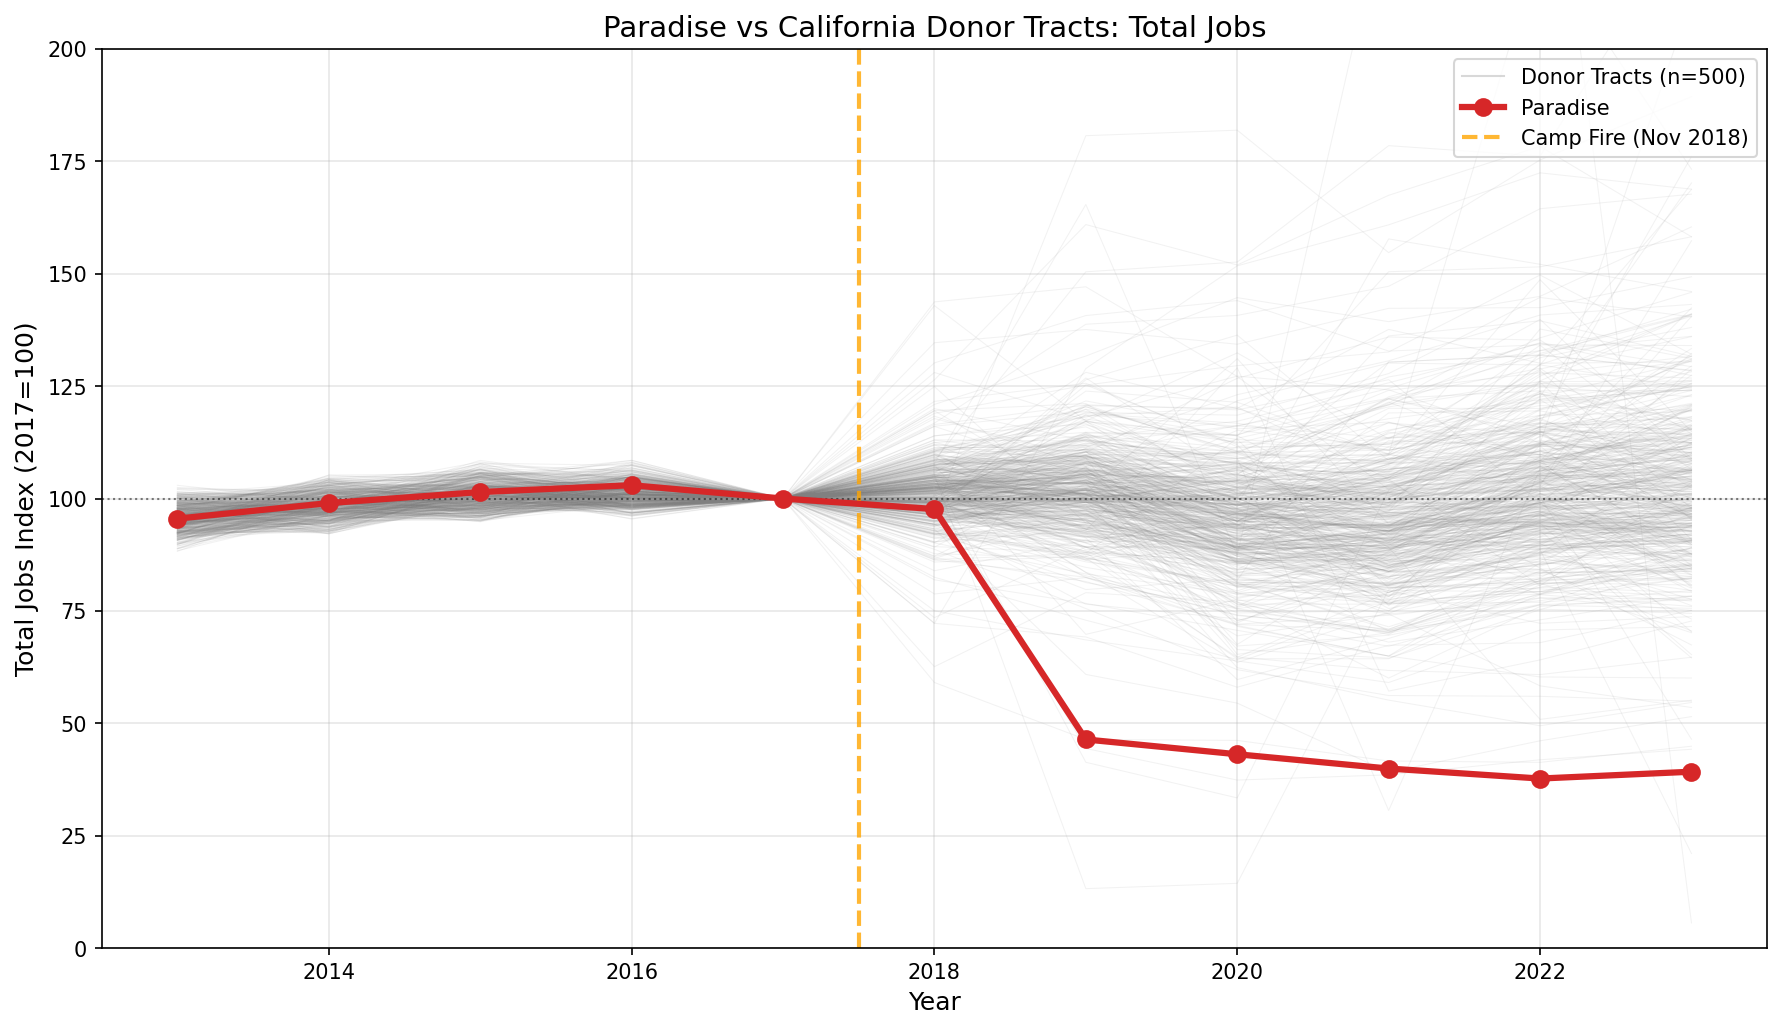
\includegraphics[width=0.85\textwidth,height=5cm,keepaspectratio]{paradise_vs_donors.png}
    \caption{Paradise employment index (red) vs.\ all California donor tracts (gray).
    Paradise's post-fire trajectory falls far outside the distribution of donors.}
  \end{figure}
\end{frame}

\begin{frame}{Placebo Tests}
  \begin{figure}
    \centering
    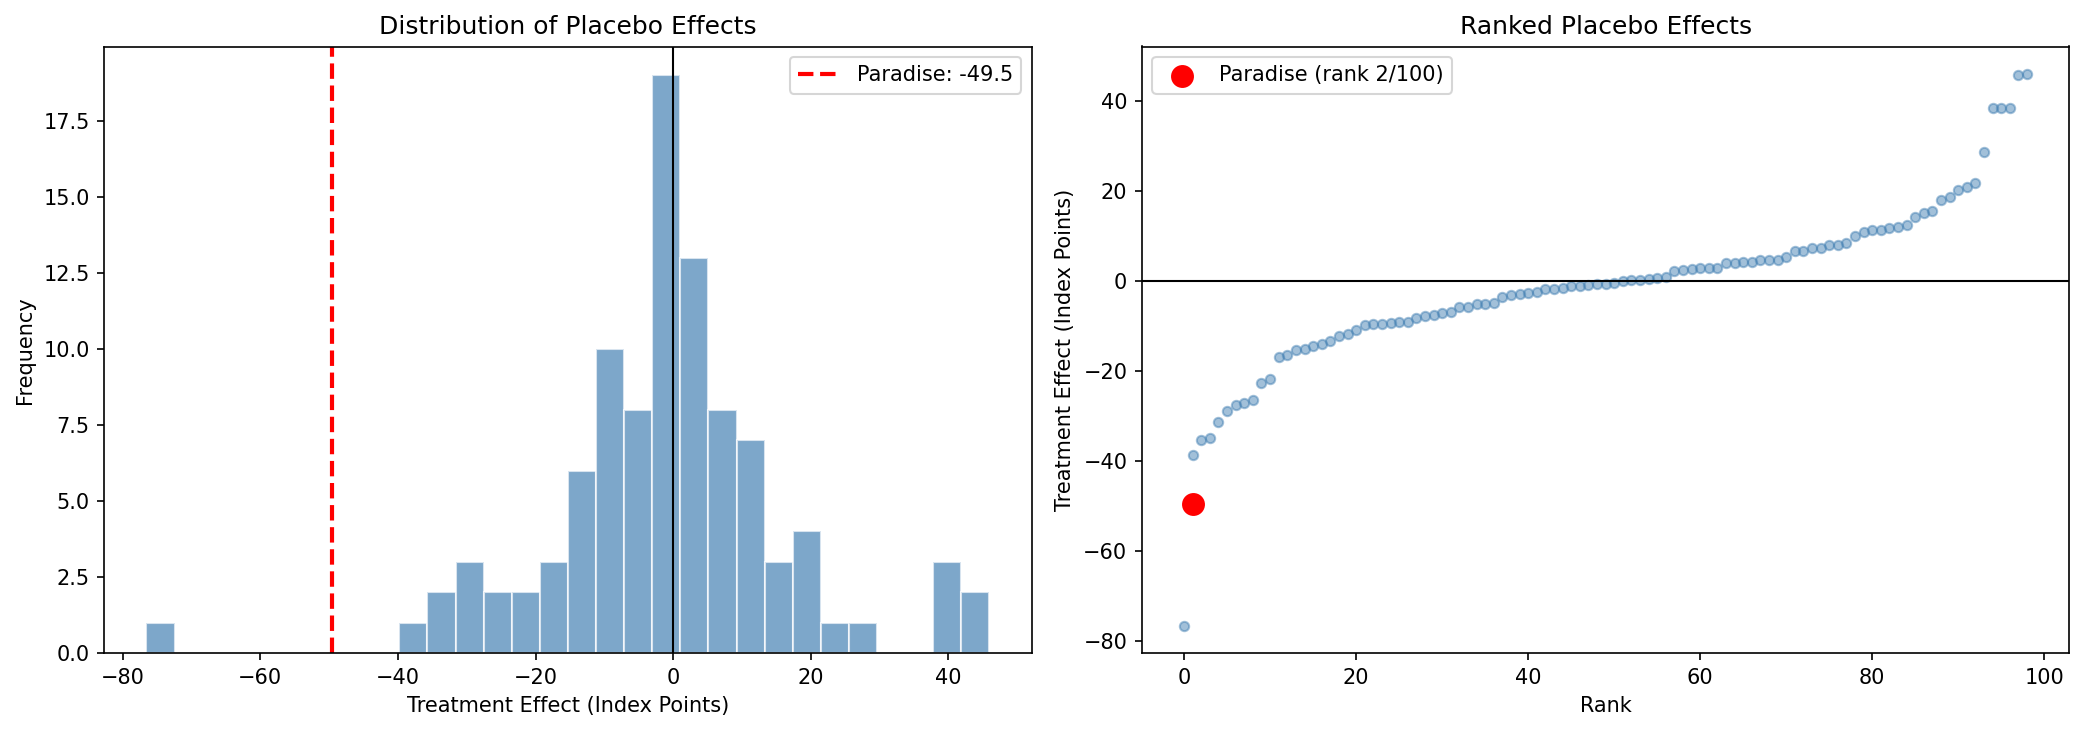
\includegraphics[width=0.75\textwidth,height=5cm,keepaspectratio]{placebo_tests.png}
    \caption{Distribution of synthetic control treatment effects for 100
    randomly selected California donor tracts (placebos). Paradise's estimated
    effect (red line) falls well below the distribution,
    confirming the magnitude is not due to chance.}
  \end{figure}
\end{frame}

% =======================================================================
\section{Spillovers}
% =======================================================================

\begin{frame}[shrink=15]{Spillover Effects: Did Chico Gain?}
  \begin{columns}[T]
    \begin{column}{0.55\textwidth}
      \begin{itemize}
        \item If displaced Paradise businesses/residents relocated to Chico,
              the Butte County \emph{control group} in the DiD would be contaminated
              --- leading to underestimates of Paradise's loss
        \item We apply synthetic control to \textbf{Chico} using Rest-of-CA donors
              to test for employment gains
        \item Result: \textbf{Chico employment barely changed}
          \begin{itemize}
            \item 2017: 49,029 jobs
            \item 2019: 50,010 jobs (+2.0\%)
            \item 2023: 48,195 jobs ($-1.7$\% from 2017)
          \end{itemize}
        \item Synthetic control gap for Chico is small and fades by 2023
      \end{itemize}
    \end{column}
    \begin{column}{0.43\textwidth}
      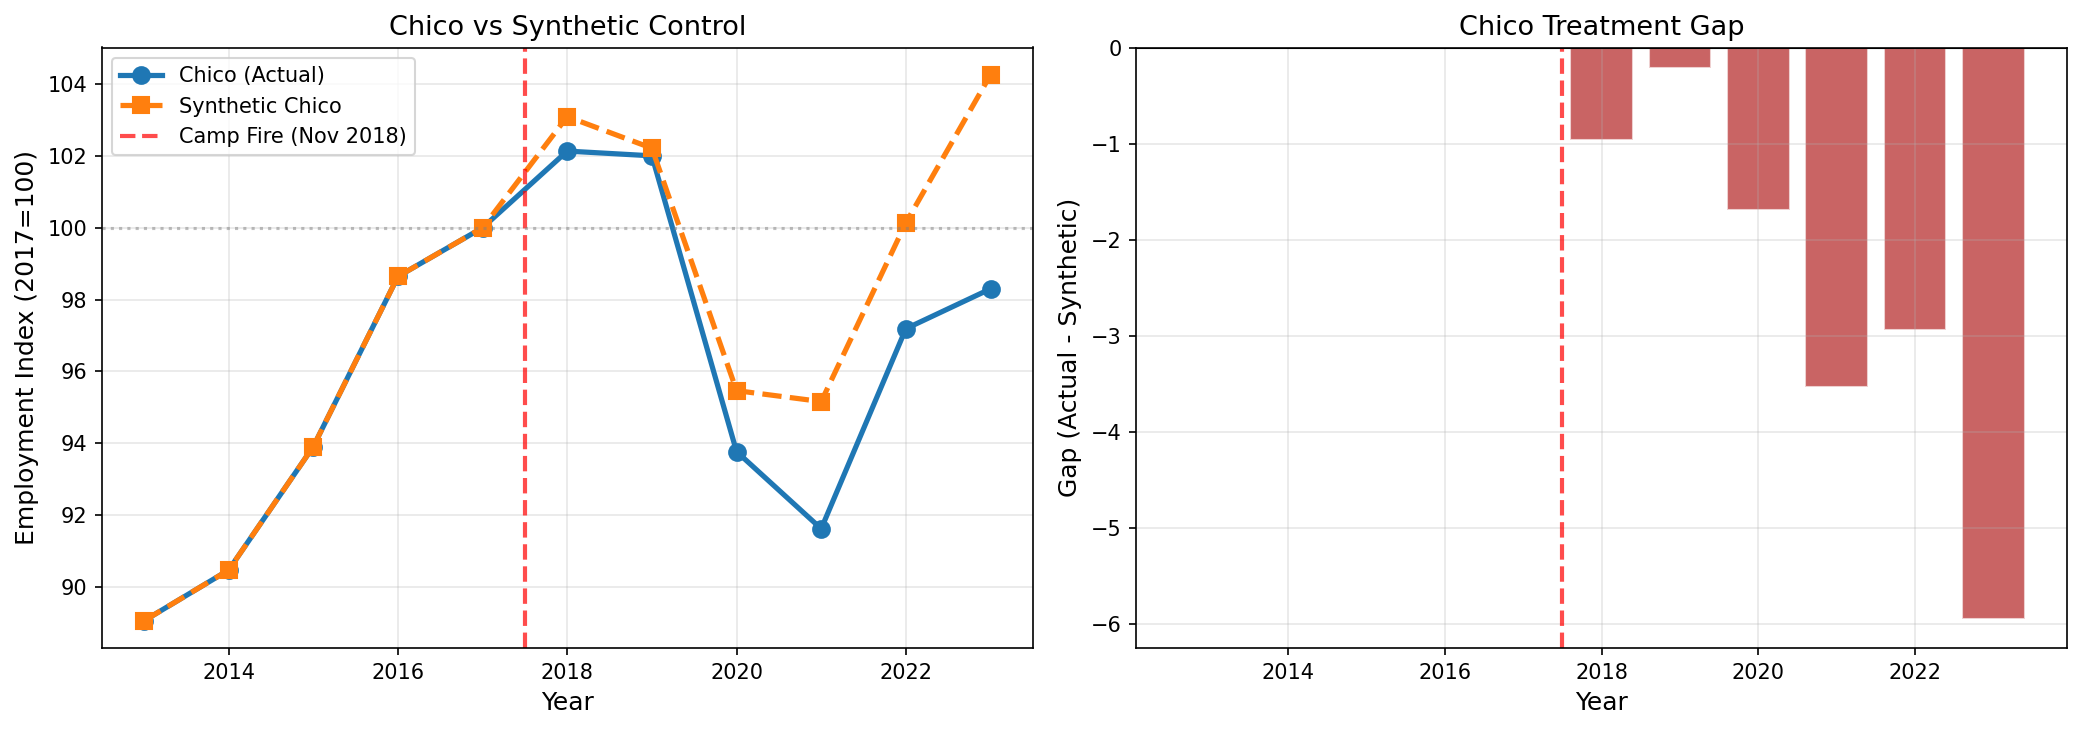
\includegraphics[width=\linewidth,height=5cm,keepaspectratio]{spillover_synthetic_chico.png}
      \captionof{figure}{\footnotesize Chico: actual vs.\ synthetic control}
    \end{column}
  \end{columns}
\end{frame}

\begin{frame}{Spillovers: Synthetic Control for Chico and Other Butte}
  \begin{columns}[T]
    \begin{column}{0.5\textwidth}
      \begin{figure}
        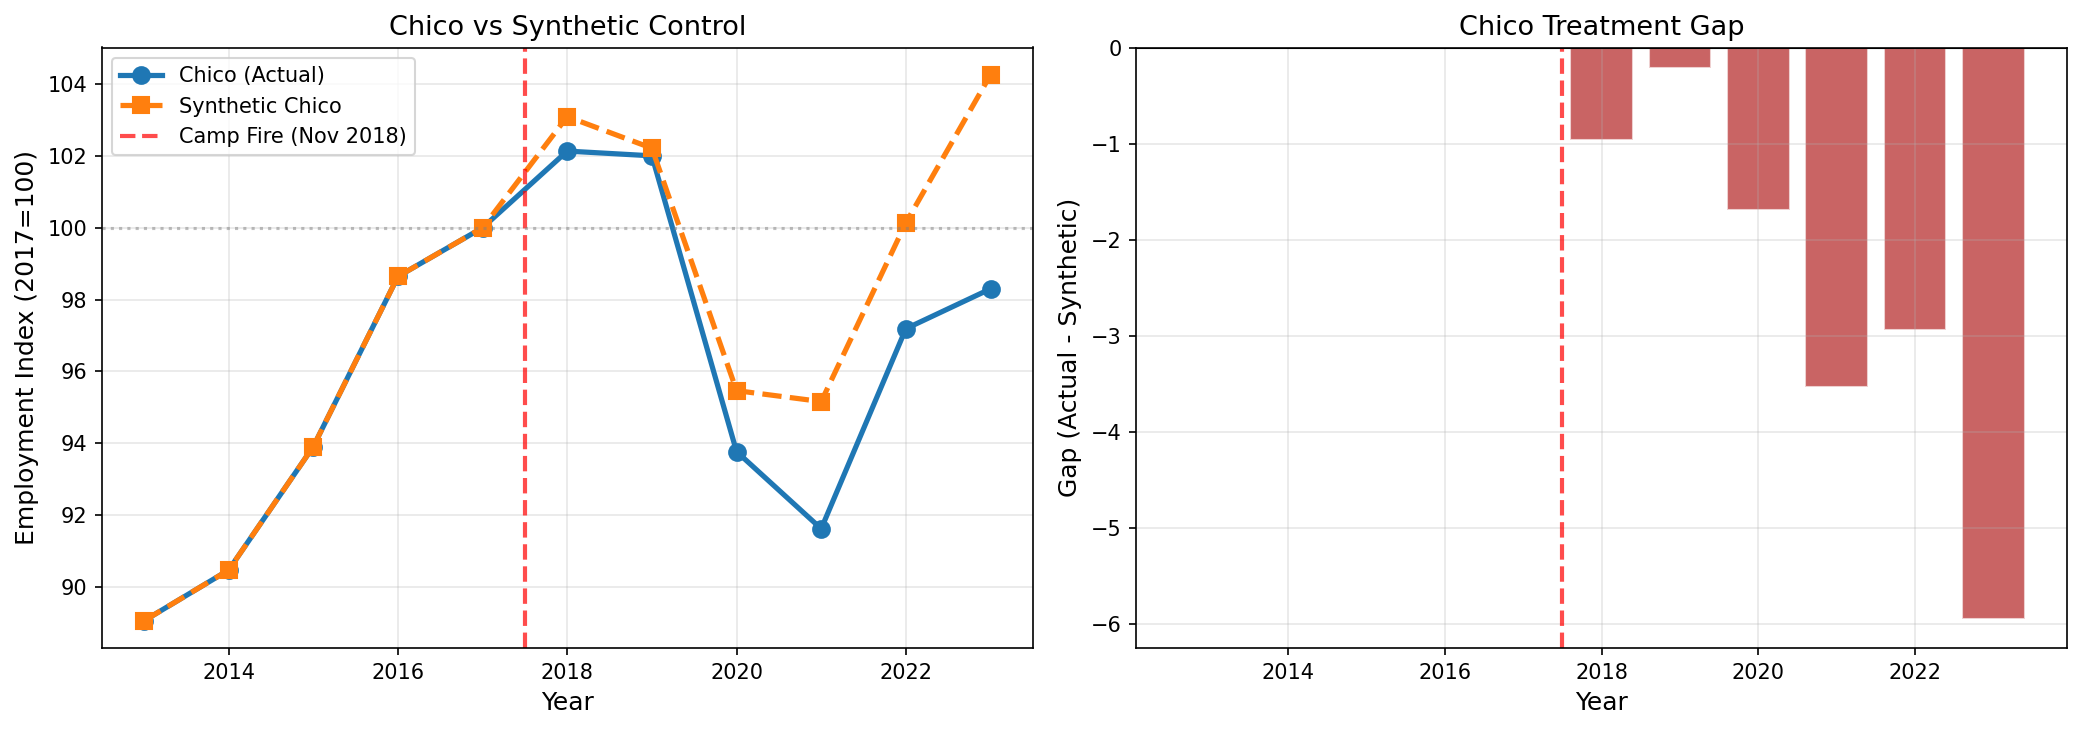
\includegraphics[width=\linewidth,height=5cm,keepaspectratio]{spillover_synthetic_chico.png}
        \caption{\footnotesize Chico: actual vs.\ synthetic}
      \end{figure}
    \end{column}
    \begin{column}{0.5\textwidth}
      \begin{figure}
        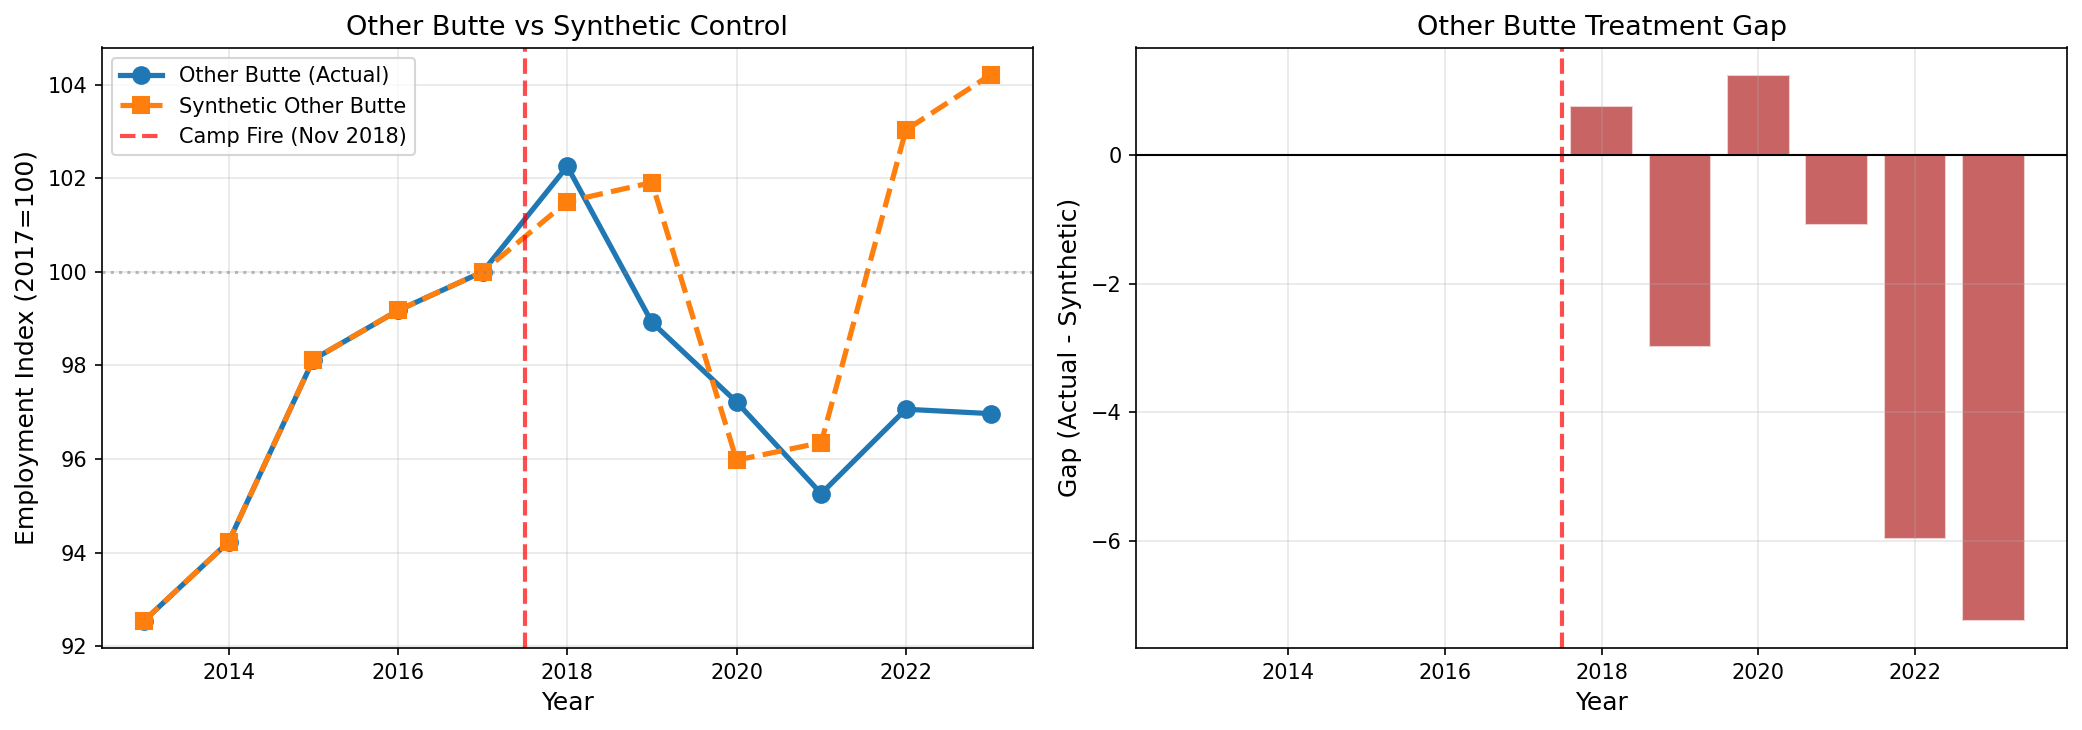
\includegraphics[width=\linewidth,height=5cm,keepaspectratio]{spillover_synthetic_other_butte.png}
        \caption{\footnotesize Other Butte: actual vs.\ synthetic}
      \end{figure}
    \end{column}
  \end{columns}
  \vspace{-0.5em}
  \footnotesize Synthetic control gaps for both zones are small and transient ---
  no evidence of sustained employment gains from Paradise displacement.
\end{frame}

\begin{frame}{Interpretation: Net Butte County Effect}
  \begin{itemize}
    \item Paradise lost roughly \textbf{3,200 jobs} (5,258 $\to$ 2,063) post-fire
    \item Chico \emph{net change}: $\approx -834$ jobs (49,029 $\to$ 48,195)
    \item Other Butte net change: $\approx -778$ jobs (25,692 $\to$ 24,914)
    \item \textbf{No evidence of significant employment displacement to Chico}
    \item DiD using Rest-of-CA as control (instead of Butte) gives similar
          point estimates, suggesting \textbf{minimal bias} in the main DiD
    \item Health care loss in Paradise ($-18.4$) did not appear to relocate
          locally --- likely reflects permanent loss of the facility base
  \end{itemize}
\end{frame}

% =======================================================================
\section{Migration}
% =======================================================================

\begin{frame}{Where Did Paradise Residents Go?}
  \begin{figure}
    \centering
    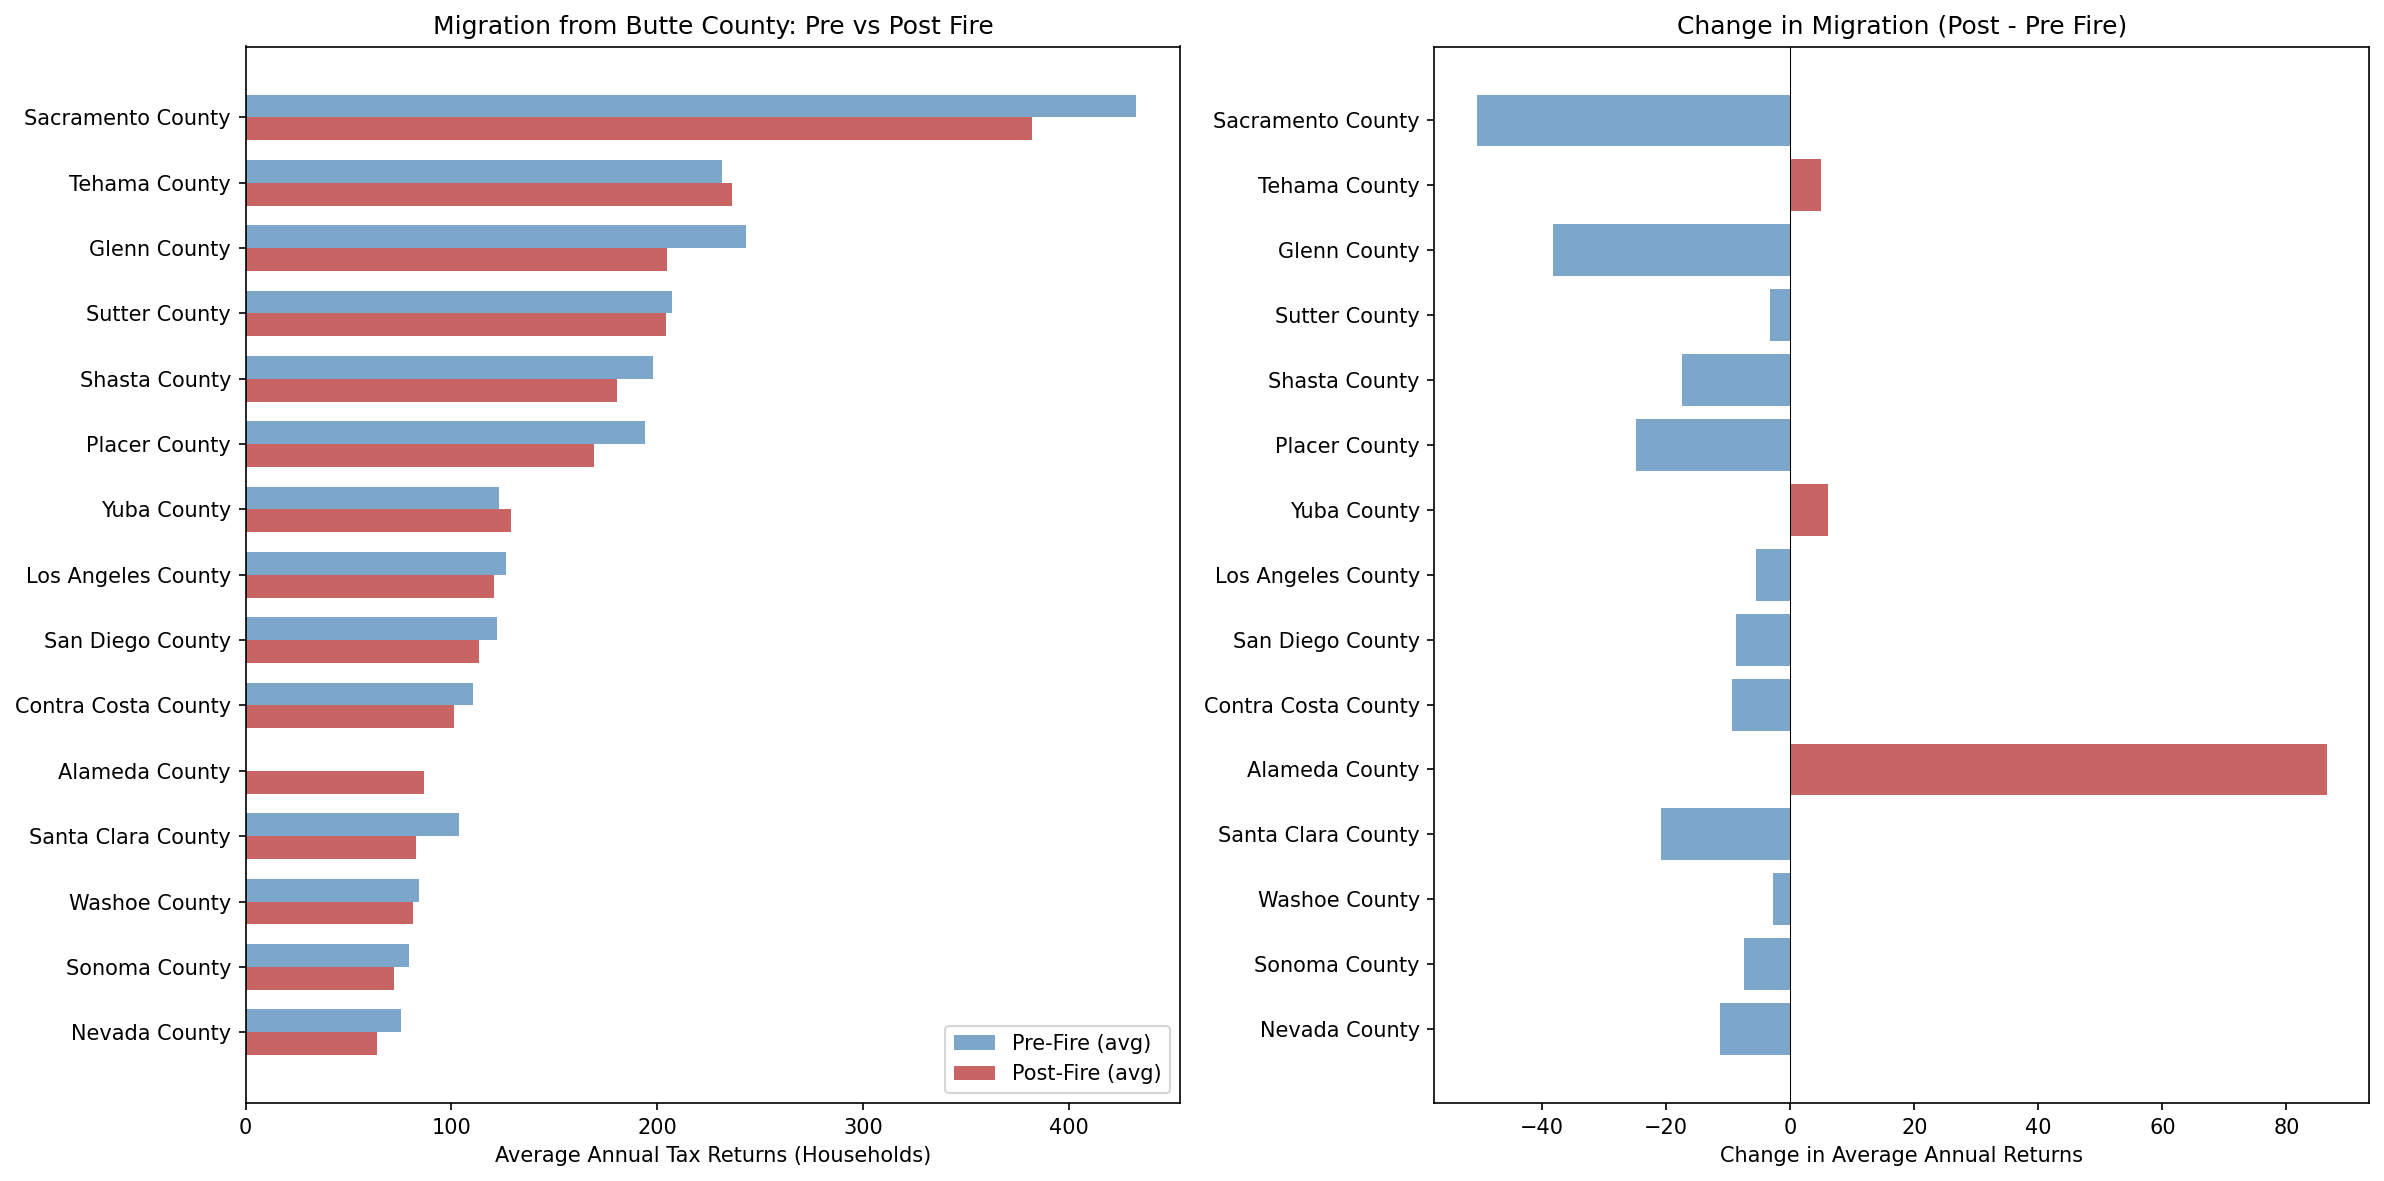
\includegraphics[width=0.85\textwidth,height=5.5cm,keepaspectratio]{migration_pre_post_comparison.png}
    \caption{IRS SOI county-to-county migration from Butte County:
    average annual outflows to top destinations, pre-fire vs.\ post-fire.}
  \end{figure}
\end{frame}

\begin{frame}{Migration: Key Patterns}
  \begin{columns}[T]
    \begin{column}{0.55\textwidth}
      \begin{figure}
        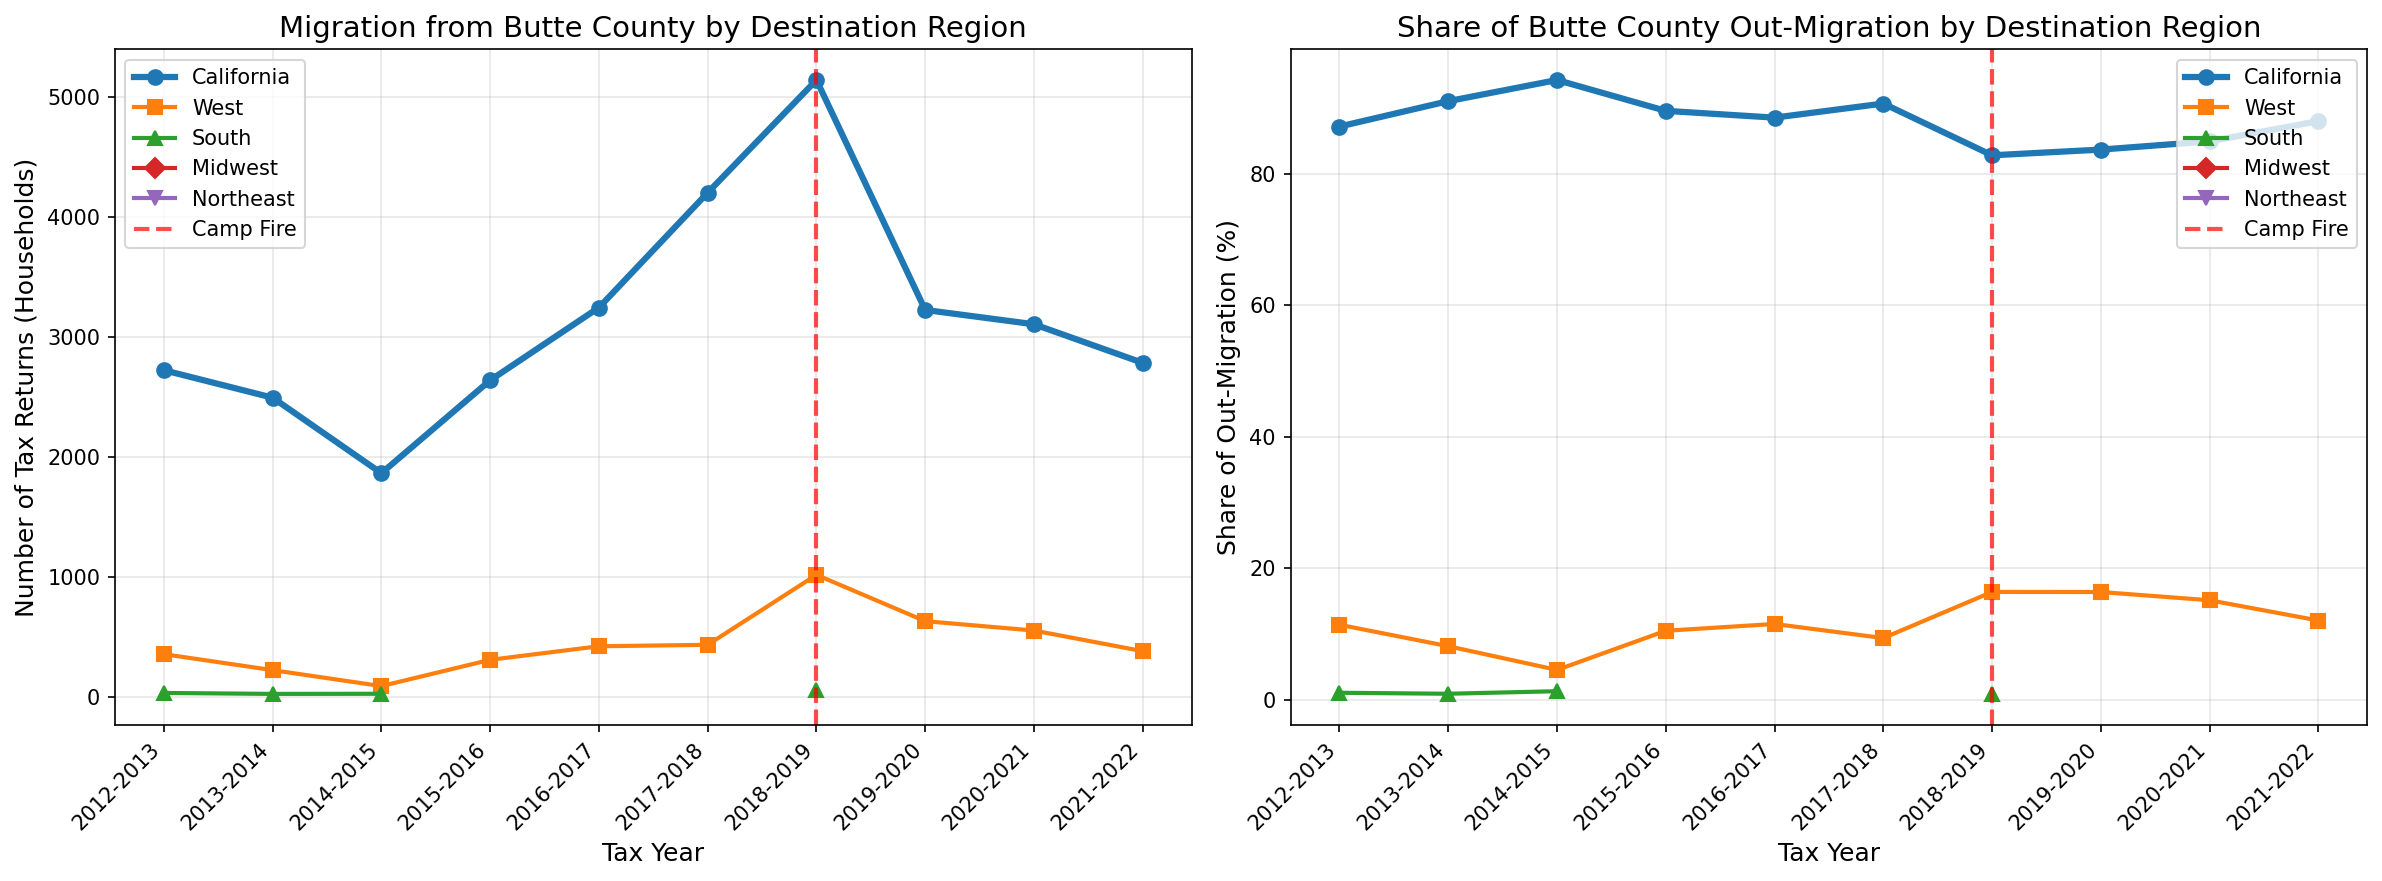
\includegraphics[width=\linewidth,height=5cm,keepaspectratio]{migration_by_region.png}
        \caption{\footnotesize Out-migration by Census region}
      \end{figure}
    \end{column}
    \begin{column}{0.43\textwidth}
      \begin{itemize}
        \item Large spike in out-migration in tax year \textbf{2018--2019}
        \item Most displacement stayed \textbf{within California}
              --- nearby Sacramento Valley counties absorbed the majority
        \item Modest increase in out-of-state flows, primarily to the
              West and South regions
        \item By 2021--2022, migration flows had normalized,
              suggesting the initial displacement shock was largely complete
      \end{itemize}
    \end{column}
  \end{columns}
\end{frame}

% =======================================================================
\section{Homelessness}
% =======================================================================

\begin{frame}{Homelessness: A Persistent Consequence}
  \begin{figure}
    \centering
    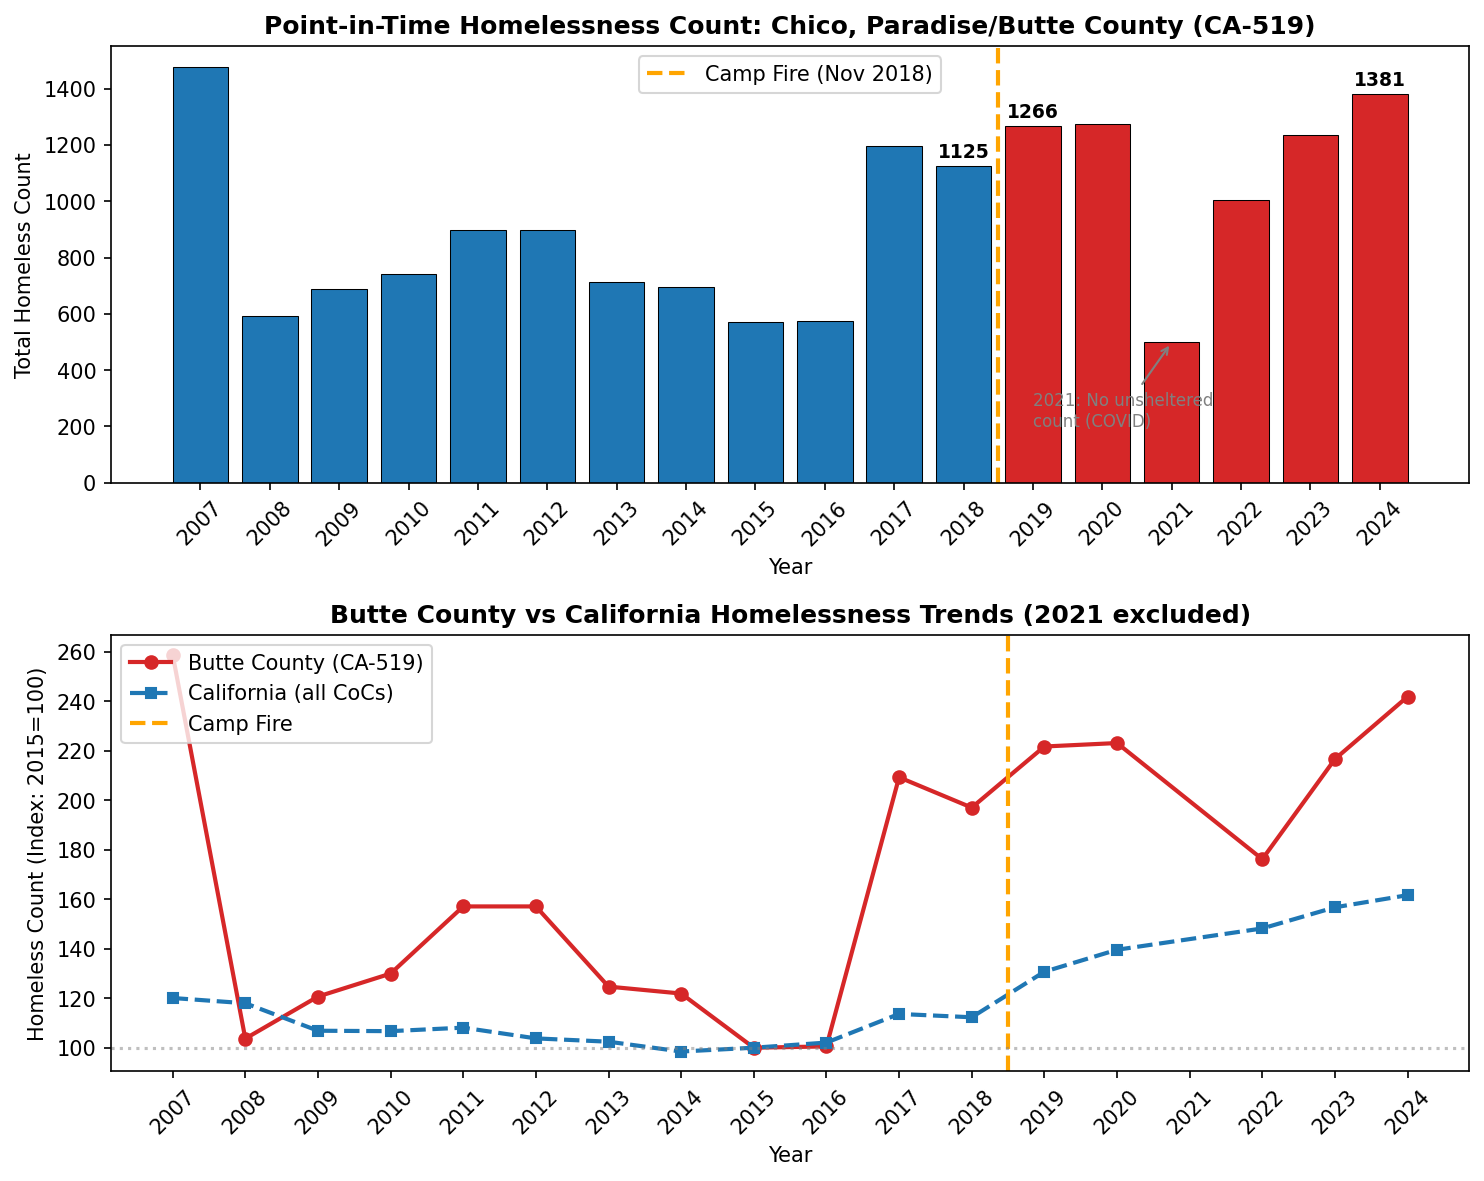
\includegraphics[width=0.8\textwidth,height=5cm,keepaspectratio]{homelessness_pit_counts.png}
    \caption{HUD Point-in-Time (PIT) homelessness counts, Butte County CoC (CA-519).
    \emph{Top}: raw counts. \emph{Bottom}: indexed to 2015 = 100, vs.\ California average.
    2021 excluded (COVID protocols suppressed unsheltered count).}
  \end{figure}
\end{frame}

\begin{frame}{Homelessness: Key Statistics}
  \begin{columns}[T]
    \begin{column}{0.55\textwidth}
      \begin{itemize}
        \item Pre-fire average (2015--2018): \textbf{866} homeless persons
        \item Post-fire average (2019--2024, excl.\ 2021): \textbf{1,233}
              (+42\%)
        \item 2019 count: 1,266 ($+12.5\%$ from 2018)
        \item 2024 count: 1,381 ($+22.8\%$ from 2018)
        \item Emergency shelter capacity more than doubled:
              274 (2018) $\to$ 641 (2024) \textbf{(+134\%)}
        \item Neighbors \emph{did not see} comparable increases:
              El Dorado $-56\%$; Yuba/Sutter $+21\%$ (2018--2024)
      \end{itemize}
    \end{column}
    \begin{column}{0.43\textwidth}
      \begin{tabular}{lrr}
        \toprule
        \textbf{CoC} & \textbf{2018} & \textbf{2024} \\
        \midrule
        Butte        & 1,125 & 1,381 \\
        Redding      & 1,149 & 2,404 \\
        Yuba/Sutter  &   765 &   928 \\
        El Dorado    &   645 &   284 \\
        Tehama       &   125 &   324 \\
        \bottomrule
      \end{tabular}
      \vspace{0.5em}
      \captionof{table}{\footnotesize Comparison CoCs, Northern CA}
    \end{column}
  \end{columns}
\end{frame}

% =======================================================================
\section{Conclusion}
% =======================================================================

\begin{frame}[shrink=5]{Summary of Findings}
  \begin{block}{Employment (DiD)}
    Paradise lost $\approx$\textbf{26.5 jobs per census block} post-fire
    (total $\approx$3,200 jobs). Effect is largest in Health Care and
    concentrated across all earnings tiers.
  \end{block}
  \begin{block}{Synthetic Control}
    By 2023, Paradise employment is \textbf{61\% below} the level predicted
    by its synthetic counterfactual. No sign of convergence.
  \end{block}
  \begin{block}{Spillovers and Migration}
    Minimal employment spillovers to Chico. Displaced residents largely
    relocated within California; out-migration normalized by 2021--2022.
  \end{block}
  \begin{block}{Homelessness}
    Post-fire homelessness is \textbf{42\% above} pre-fire average,
    with emergency shelter capacity more than doubled by 2024.
  \end{block}
\end{frame}

\begin{frame}{Discussion}
  \begin{itemize}
    \item The Camp Fire represents a \textbf{total destruction} event ---
          employment has not recovered six years later
    \item The \textbf{health care sector} (clinics, hospital) was the single
          largest employer; its loss is not offset by Chico's capacity
    \item \textbf{Construction} is the one bright spot, consistent with
          ongoing rebuilding, but it has not pulled broader recovery
    \item Homelessness data suggest a substantial share of the displaced
          population has not secured stable housing
    \item \textbf{Policy implication}: Wildfire economic recovery requires
          targeted support for healthcare infrastructure and
          affordable housing, not just physical rebuilding
  \end{itemize}
\end{frame}

\begin{frame}{Future Work}
  \begin{itemize}
    \item Commute analysis (LODES OD): Did Paradise residents continue
          working in Butte County from new residential locations?
    \item USPS vacancy data: Residential vs.\ business vacancy dynamics
          across the county ($\to$ housing supply recovery timeline)
    \item Extend migration analysis to 2022--2023 IRS data when available
    \item Wage effects: match LODES to Quarterly Census of Employment
          and Wages (QCEW) for wage-per-job analysis
    \item Comparison to other total-destruction wildfire events
          (e.g., Lahaina 2023) and hurricane disasters
  \end{itemize}
\end{frame}

% --- Appendix -----------------------------------------------------------
\appendix

\begin{frame}{Appendix: DiD Results --- Residence Area (RAC)}
  \begin{table}
    \centering
    \footnotesize
    \begin{tabular}{lrrr}
      \toprule
      \textbf{Outcome} & \textbf{DiD Coef.} & \textbf{Std.\ Err.} & \textbf{p-value} \\
      \midrule
      Total Jobs          & $-24.7$ & $2.3$ & $<0.001$\,*** \\
      \midrule
      Retail Trade        & $-3.0$  & $0.2$ & $<0.001$\,*** \\
      Health Care         & $-7.6$  & $0.8$ & $<0.001$\,*** \\
      Accommodation \& Food & $-2.2$ & $0.1$ & $<0.001$\,*** \\
      Construction        & $-1.1$  & $0.2$ & $<0.001$\,*** \\
      Education           & $-2.0$  & $0.3$ & $<0.001$\,*** \\
      Public Admin        & $-1.2$  & $0.2$ & $<0.001$\,*** \\
      \midrule
      Low Earnings        & $-7.0$  & $0.7$ & $<0.001$\,*** \\
      Medium Earnings     & $-8.6$  & $0.7$ & $<0.001$\,*** \\
      High Earnings       & $-9.1$  & $0.9$ & $<0.001$\,*** \\
      \bottomrule
    \end{tabular}
    \caption{DiD estimates, RAC (residence). $N = 36{,}283$. SE clustered by tract.}
  \end{table}
\end{frame}

\begin{frame}{Appendix: Synthetic Control Data}
  \begin{table}
    \centering
    \footnotesize
    \begin{tabular}{lrrr}
      \toprule
      \textbf{Year} & \textbf{Paradise} & \textbf{Synthetic} & \textbf{Gap} \\
      \midrule
      2017 & 100.0 & 100.0 &   0.0 \\
      2018 &  97.7 & 102.9 &  $-5.2$ \\
      2019 &  46.4 & 101.4 & $-55.0$ \\
      2020 &  43.1 &  94.1 & $-51.0$ \\
      2021 &  39.9 &  96.2 & $-56.2$ \\
      2022 &  37.7 & 103.1 & $-65.4$ \\
      2023 &  39.2 & 103.5 & $-64.3$ \\
      \bottomrule
    \end{tabular}
    \caption{Synthetic control results (WAC, total jobs). Index: 2017 = 100.
    Pre-treatment RMSE $\approx 0$ (near-perfect fit).}
  \end{table}
\end{frame}

\begin{frame}{Appendix: Employment by Zone (Raw Counts)}
  \begin{table}
    \centering
    \footnotesize
    \begin{tabular}{lrrrr}
      \toprule
      \textbf{Year} & \textbf{Paradise} & \textbf{Chico} & \textbf{Other Butte} & \textbf{Rest of CA (000s)} \\
      \midrule
      2013 &  5,023 & 43,665 & 23,777 & 15,111 \\
      2017 &  5,258 & 49,029 & 25,692 & 16,734 \\
      2018 &  5,135 & 50,075 & 26,271 & 17,077 \\
      2019 &  2,440 & 50,010 & 25,415 & 17,291 \\
      2021 &  2,100 & 44,921 & 24,475 & 16,419 \\
      2023 &  2,063 & 48,195 & 24,914 & 17,780 \\
      \bottomrule
    \end{tabular}
    \caption{Total workplace jobs (WAC) by geographic zone.
    Paradise job count approximately halved in 2018--2019 and has not recovered.}
  \end{table}
\end{frame}

\end{document}
